% Author: Izaak Neutelings (July, 2017)

\documentclass[border=3pt,tikz]{standalone}
\usepackage{tikz}

% colors
\definecolor{mylightred}{RGB}{255,210,210}
\definecolor{myred}{RGB}{200,100,100}
\definecolor{mydarkred}{RGB}{140,40,40}
\definecolor{mylightblue}{RGB}{220,228,255}
\definecolor{myblue}{RGB}{183,191,229}
\definecolor{mydarkblue}{RGB}{50,70,190}

\begin{document}



% RUTHERFORD MODEL - atom model with central charge
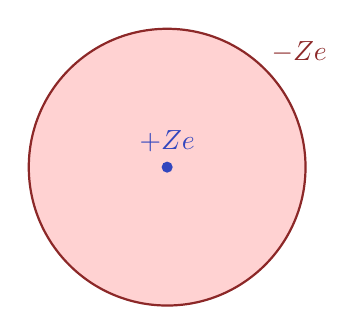
\begin{tikzpicture}[scale=1]
  \coordinate (O)  at (0,0);
  \draw[mylightred,fill]         (O) circle (50pt);
  \draw[mydarkred,thick]         (O) circle (50pt) node[above right=34pt] {$-Ze$};
  \fill[radius=2.0pt,mydarkblue] (O) circle node[above=2pt] {$+Ze$};
\end{tikzpicture}



% RUTHERFORD MODEL - atom model with central charge and corpuscles
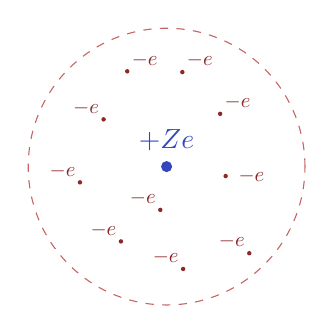
\begin{tikzpicture}[scale=1]
  \coordinate (O)  at (0,0);
  \draw[myred,dashed]            (O) circle (50pt);
  \fill[radius=2.0pt,mydarkblue] (O) circle node[above=2pt] {$+Ze$};
  \fill[radius=0.8pt,mydarkred]
    ( 0.20, 1.20)  circle node[above right=-1pt,scale=0.75] {$-e$}
    ( 0.68, 0.67)  circle node[above right=-1pt,scale=0.75] {$-e$}
    ( 1.05,-1.10)  circle node[above left =-1pt,scale=0.75] {$-e$}
    ( 0.75,-0.12)  circle node[      right= 2pt,scale=0.75] {$-e$}
    ( 0.21,-1.30)  circle node[above left =-1pt,scale=0.75] {$-e$}
    (-0.80, 0.60)  circle node[above left =-1pt,scale=0.75] {$-e$}
    (-0.50, 1.21)  circle node[above right=-1pt,scale=0.75] {$-e$}
    (-0.08,-0.55)  circle node[above left =-1pt,scale=0.75] {$-e$}
    (-0.58,-0.95)  circle node[above left =-1pt,scale=0.75] {$-e$}
    (-1.10,-0.20)  circle node[above left =-1pt,scale=0.75] {$-e$};
\end{tikzpicture}



% THOMSON MODEL - atom model with corpuscles (electrons) in uniformly, positively charged sphere
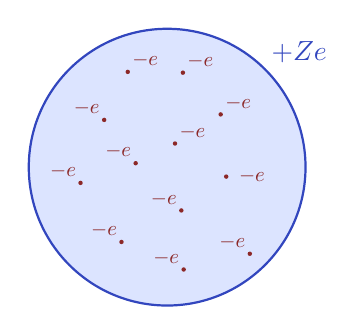
\begin{tikzpicture}[scale=1]
  \coordinate (O)  at (0,0);
  \draw[mylightblue,fill] (O) circle (50pt);
  \draw[mydarkblue,thick] (O) circle (50pt) node[above right=34pt] {$+Ze$};
  \fill[radius=0.8pt,mydarkred]
    ( 0.20, 1.20)  circle node[above right=-1pt,scale=0.75] {$-e$}
    ( 0.10, 0.30)  circle node[above right=-1pt,scale=0.75] {$-e$}
    ( 0.68, 0.67)  circle node[above right=-1pt,scale=0.75] {$-e$}
    ( 1.05,-1.10)  circle node[above left =-1pt,scale=0.75] {$-e$}
    ( 0.75,-0.12)  circle node[      right= 2pt,scale=0.75] {$-e$}
    ( 0.21,-1.30)  circle node[above left =-1pt,scale=0.75] {$-e$}
    ( 0.18,-0.55)  circle node[above left =-1pt,scale=0.75] {$-e$}
    (-0.80, 0.60)  circle node[above left =-1pt,scale=0.75] {$-e$}
    (-0.50, 1.21)  circle node[above right=-1pt,scale=0.75] {$-e$}
    (-0.40, 0.05)  circle node[above left =-1pt,scale=0.75] {$-e$}
    (-0.58,-0.95)  circle node[above left =-1pt,scale=0.75] {$-e$}
    (-1.10,-0.20)  circle node[above left =-1pt,scale=0.75] {$-e$};
\end{tikzpicture}



\end{document}
